% $Id: getdp.tex,v 1.14 2001-06-15 12:21:46 geuzaine Exp $

\newcommand{\smallgetdp}[1]
   {\background{7\semcm}{4.2\semcm}{\scalebox{0.3}{\input{#1}}}}

% ---------------------------------------------------------------------------
\part{GetDP}
% ---------------------------------------------------------------------------

\begin{slide}

\slidepagestyle{none}

\begin{center}
\bigtitle{GetDP --- A general software environment for the treatment of
          discrete problems}\\
\ifnum\fulltitle=1\par\bigskip\bigskip
\mediumtitle{Patrick Dular and Christophe Geuzaine}\\
\bigskip
\smalltitle{Department of Electrical Engineering}\\
\smalltitle{Montefiore Institute B28, Sart Tilman Campus}\\
\smalltitle{University of Li�ge}\\
\smalltitle{B-4000 Li�ge (BELGIUM)}
\fi
\end{center}

\end{slide}

% ---------------------------------------------------------------------------

\chapter{An environment open to various couplings}

\begin{slide}

Any coupling between 
\begin{slideitemize}
\item \emph{Physical} problems (electromagnetic, thermal, mechanical, ...)
\item \emph{Numerical} methods (finite element methods, integral methods, ...)
\item \emph{Geometries} (1D, 2D, 3D)
\item \emph{Time} states (static, harmonic, transient)
\end{slideitemize}

How?
\begin{slideitemize}
\item Clear \emph{mathematical} definitions/structure
\item Directly transcribed into 10 interdependent \emph{objects}
\end{slideitemize}

\end{slide}

% ---------------------------------------------------------------------------

\chapter{Definition of discrete problems}

\begin{slide}

\begin{center}
Copy of the formal mathematical expression of problems in \emph{text data
files} (``\code{.pro} files'')
\end{center}

\begin{center}
\scalebox{0.54}{\begin{picture}(0,0)%
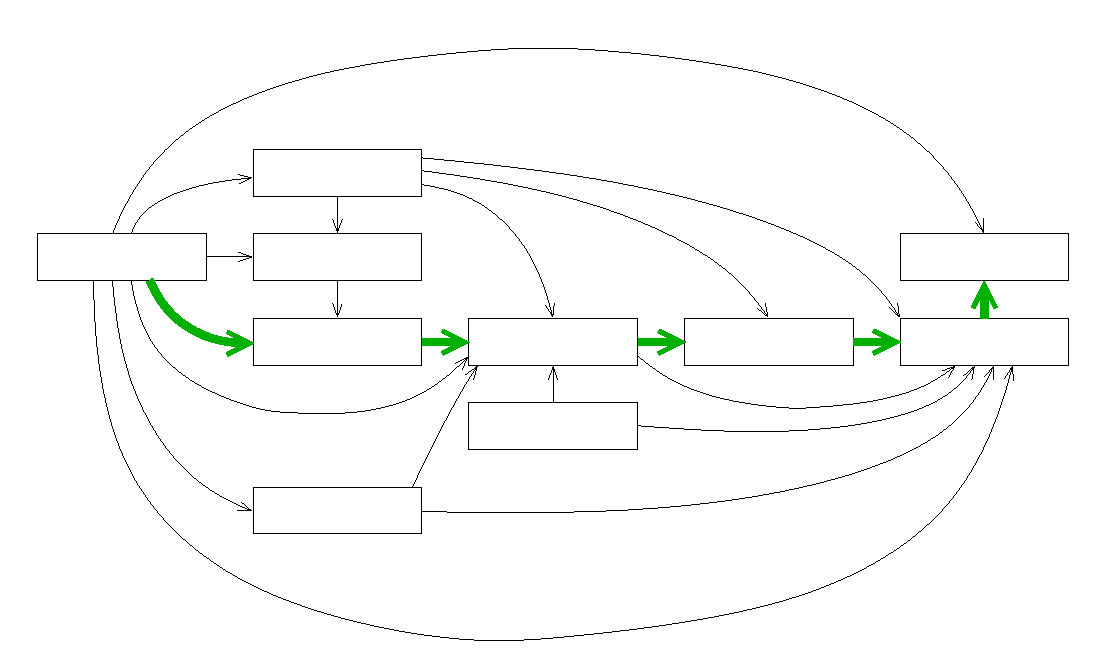
\includegraphics{getdp-struct}%
\end{picture}%
\setlength{\unitlength}{3947sp}%
%
\begingroup\makeatletter\ifx\SetFigFont\undefined%
\gdef\SetFigFont#1#2#3#4#5{%
  \reset@font\fontsize{#1}{#2pt}%
  \fontfamily{#3}\fontseries{#4}\fontshape{#5}%
  \selectfont}%
\fi\endgroup%
\begin{picture}(8552,4992)(300,-6402)
\put(1126,-3361){\makebox(0,0)[b]{\smash{\SetFigFont{10}{12.0}{\rmdefault}{\mddefault}{\updefault}{\color[rgb]{0,0,0}\code{Group}}%
}}}
\put(2851,-2686){\makebox(0,0)[b]{\smash{\SetFigFont{10}{12.0}{\rmdefault}{\mddefault}{\updefault}{\color[rgb]{0,0,0}\code{Function}}%
}}}
\put(2851,-3361){\makebox(0,0)[b]{\smash{\SetFigFont{10}{12.0}{\rmdefault}{\mddefault}{\updefault}{\color[rgb]{0,0,0}\code{Constraint}}%
}}}
\put(2851,-4036){\makebox(0,0)[b]{\smash{\SetFigFont{10}{12.0}{\rmdefault}{\mddefault}{\updefault}{\color[rgb]{0,0,0}\code{FunctionSpace}}%
}}}
\put(2851,-5386){\makebox(0,0)[b]{\smash{\SetFigFont{10}{12.0}{\rmdefault}{\mddefault}{\updefault}{\color[rgb]{0,0,0}\code{Jacobian}}%
}}}
\put(4576,-4711){\makebox(0,0)[b]{\smash{\SetFigFont{10}{12.0}{\rmdefault}{\mddefault}{\updefault}{\color[rgb]{0,0,0}\code{Integration}}%
}}}
\put(4576,-4036){\makebox(0,0)[b]{\smash{\SetFigFont{10}{12.0}{\rmdefault}{\mddefault}{\updefault}{\color[rgb]{0,0,0}\code{Formulation}}%
}}}
\put(6301,-4036){\makebox(0,0)[b]{\smash{\SetFigFont{10}{12.0}{\rmdefault}{\mddefault}{\updefault}{\color[rgb]{0,0,0}\code{Resolution}}%
}}}
\put(8026,-3361){\makebox(0,0)[b]{\smash{\SetFigFont{10}{12.0}{\rmdefault}{\mddefault}{\updefault}{\color[rgb]{0,0,0}\code{PostOperation}}%
}}}
\put(8026,-4036){\makebox(0,0)[b]{\smash{\SetFigFont{10}{12.0}{\rmdefault}{\mddefault}{\updefault}{\color[rgb]{0,0,0}\code{PostProcessing}}%
}}}
\end{picture}
}
\end{center}

\end{slide}

\begin{slide}

\begin{center}
Particular data of a problem\\
\medskip
\scalebox{0.54}{\begin{picture}(0,0)%
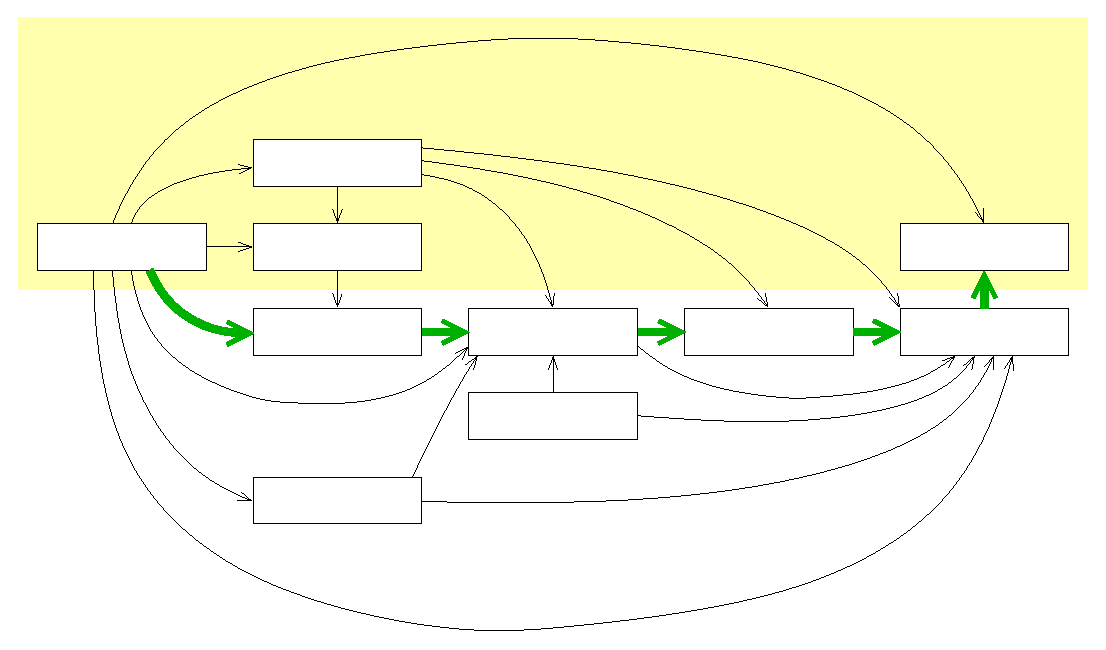
\includegraphics{getdp-struct-box}%
\end{picture}%
\setlength{\unitlength}{3947sp}%
%
\begingroup\makeatletter\ifx\SetFigFont\undefined%
\gdef\SetFigFont#1#2#3#4#5{%
  \reset@font\fontsize{#1}{#2pt}%
  \fontfamily{#3}\fontseries{#4}\fontshape{#5}%
  \selectfont}%
\fi\endgroup%
\begin{picture}(8552,4917)(300,-6402)
\put(1126,-3361){\makebox(0,0)[b]{\smash{\SetFigFont{10}{12.0}{\rmdefault}{\mddefault}{\updefault}{\color[rgb]{0,0,0}\code{Group}}%
}}}
\put(2851,-2686){\makebox(0,0)[b]{\smash{\SetFigFont{10}{12.0}{\rmdefault}{\mddefault}{\updefault}{\color[rgb]{0,0,0}\code{Function}}%
}}}
\put(2851,-3361){\makebox(0,0)[b]{\smash{\SetFigFont{10}{12.0}{\rmdefault}{\mddefault}{\updefault}{\color[rgb]{0,0,0}\code{Constraint}}%
}}}
\put(2851,-4036){\makebox(0,0)[b]{\smash{\SetFigFont{10}{12.0}{\rmdefault}{\mddefault}{\updefault}{\color[rgb]{0,0,0}\code{FunctionSpace}}%
}}}
\put(2851,-5386){\makebox(0,0)[b]{\smash{\SetFigFont{10}{12.0}{\rmdefault}{\mddefault}{\updefault}{\color[rgb]{0,0,0}\code{Jacobian}}%
}}}
\put(4576,-4711){\makebox(0,0)[b]{\smash{\SetFigFont{10}{12.0}{\rmdefault}{\mddefault}{\updefault}{\color[rgb]{0,0,0}\code{Integration}}%
}}}
\put(4576,-4036){\makebox(0,0)[b]{\smash{\SetFigFont{10}{12.0}{\rmdefault}{\mddefault}{\updefault}{\color[rgb]{0,0,0}\code{Formulation}}%
}}}
\put(6301,-4036){\makebox(0,0)[b]{\smash{\SetFigFont{10}{12.0}{\rmdefault}{\mddefault}{\updefault}{\color[rgb]{0,0,0}\code{Resolution}}%
}}}
\put(8026,-3361){\makebox(0,0)[b]{\smash{\SetFigFont{10}{12.0}{\rmdefault}{\mddefault}{\updefault}{\color[rgb]{0,0,0}\code{PostOperation}}%
}}}
\put(8026,-4036){\makebox(0,0)[b]{\smash{\SetFigFont{10}{12.0}{\rmdefault}{\mddefault}{\updefault}{\color[rgb]{0,0,0}\code{PostProcessing}}%
}}}
\end{picture}
}\\
\medskip
Method of resolution (``black box'')
\end{center}

\end{slide}

% ---------------------------------------------------------------------------

\smallgetdp{fig/getdp-struct-group.tex}

\chapter{\code{Group}: defining topological entities}

\begin{slide}

\mybox{colbox}{11\semcm}{
  \begin{slideitemize}
  \item Regions
  \item Functions on Regions (nodes, edges, edges of tree, ...)
  \end{slideitemize}
}

\bigskip
\begin{syntax}
Air = Region[1]; \CC{elementary group (linked with the mesh)}
Core = Region[2];
Omega = Region[\{Air, Core\}];
Nodes = NodesOf[Omega]; \CC{function group}
\end{syntax}

\end{slide}

% ---------------------------------------------------------------------------

\smallgetdp{fig/getdp-struct-function.tex}

\chapter{\code{Function}: defining expressions}

\begin{slide}

\mybox{colbox}{11\semcm}{
  \begin{slideitemize}
  \item Physical characteristics
  \item Time functions
  \item Various other functions (natural constraints, ...)
  \end{slideitemize}
}

\bigskip
\begin{syntax}
mu0 = 4.e-7*Pi; f = 50; \CC{constants}
mu[Air] = mu0; 
mu[Core] = mu0 + 1/(100+100*$1^6); \CC{argument ($1 <- b)}
TimeFct[] = Cos[2*Pi*f*$Time] * Exp[-$Time/0.012]; \CC{current value}
\end{syntax}

\end{slide}

% ---------------------------------------------------------------------------

\smallgetdp{fig/getdp-struct-constraint.tex}

\chapter{\code{Constraint}: specifying constraints}

\begin{slide}

\mybox{colbox}{11\semcm}{
  \begin{slideitemize}
  \item Boundary conditions (classical, connection)
  \item Initial conditions
  \item Topology of circuits with lumped elements
  \item Other constraints (on local and global quantities)
  \end{slideitemize}
}

\bigskip
\begin{syntax}
\{ Name Dirichlet; Type Assign; \CC{boundary conditions}
  Case \{ \{ Region Surface0; Value 0; \}
         \{ Region Surface1; Value 1; \} \}
\}
\end{syntax}

\end{slide}

\background{7\semcm}{-2.5\semcm}{\scalebox{0.65}{\begin{picture}(0,0)%
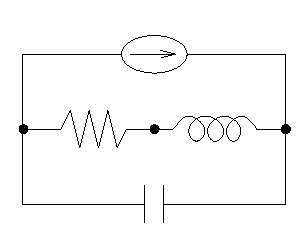
\includegraphics{getdp-rlccircuit}%
\end{picture}%
\setlength{\unitlength}{3947sp}%
%
\begingroup\makeatletter\ifx\SetFigFont\undefined%
\gdef\SetFigFont#1#2#3#4#5{%
  \reset@font\fontsize{#1}{#2pt}%
  \fontfamily{#3}\fontseries{#4}\fontshape{#5}%
  \selectfont}%
\fi\endgroup%
\begin{picture}(2387,1794)(1923,-4573)
\put(4310,-3856){\makebox(0,0)[lb]{\smash{\SetFigFont{10}{12.0}{\rmdefault}{\mddefault}{\updefault}{\color[rgb]{0,0,0}$2$}%
}}}
\put(3601,-3586){\makebox(0,0)[lb]{\smash{\SetFigFont{10}{12.0}{\rmdefault}{\mddefault}{\updefault}{\color[rgb]{0,0,0}$L_1$}%
}}}
\put(3076,-2944){\makebox(0,0)[lb]{\smash{\SetFigFont{10}{12.0}{\rmdefault}{\mddefault}{\updefault}{\color[rgb]{0,0,0}$E_1$}%
}}}
\put(2615,-3527){\makebox(0,0)[lb]{\smash{\SetFigFont{10}{12.0}{\rmdefault}{\mddefault}{\updefault}{\color[rgb]{0,0,0}$R_1$}%
}}}
\put(1923,-3869){\makebox(0,0)[lb]{\smash{\SetFigFont{10}{12.0}{\rmdefault}{\mddefault}{\updefault}{\color[rgb]{0,0,0}$1$}%
}}}
\put(3119,-3710){\makebox(0,0)[lb]{\smash{\SetFigFont{10}{12.0}{\rmdefault}{\mddefault}{\updefault}{\color[rgb]{0,0,0}$3$}%
}}}
\put(3086,-4138){\makebox(0,0)[lb]{\smash{\SetFigFont{10}{12.0}{\rmdefault}{\mddefault}{\updefault}{\color[rgb]{0,0,0}$C_1$}%
}}}
\end{picture}
}}

\begin{slide}

\begin{syntax}
\{ Name Current; Type Assign; \CC{constraints on global quantities}
  Case \{ 
    \{ Region Inductor1; Value 1000; TimeFunction TimeFct[]; \} 
  \} 
\}

\{ Name ElectricalCircuit; Type Network; \CC{circuit}
  Case Circuit1 \{ 
    \{ Region E1; Branch \{1,2\}; \}
    \{ Region R1; Branch \{1,3\}; \}
    \{ Region L1; Branch \{3,2\}; \}
    \{ Region C1; Branch \{1,2\}; \}
  \}
\}
\end{syntax}

\end{slide}


% ---------------------------------------------------------------------------

\smallgetdp{fig/getdp-struct-functionspace.tex}

\chapter{\code{FunctionSpace}: building function spaces}

\begin{slide}

\mybox{colbox}{11\semcm}{
  \begin{slideitemize}
  \item Various quantity types (0, 1, 2, 3-forms, scalar, vector)
  \item Various basis functions (associated with nodes, edges, facets,
  volumes) of various orders
  \item Coupling of fields and potentials ($T$-$\Omega$, $\vec{h}$-$\phi$,
  $\vec{a}$-$v$, ...)
  \item Definition of global quantities (fluxes, circulations: current,
  voltage, m.m.f., ...)
  \item Essential constraints (boundary and gauge conditions, ...)
  \end{slideitemize}
}

\rput(0.75\textwidth,4\semcm){\begin{picture}(0,0)%
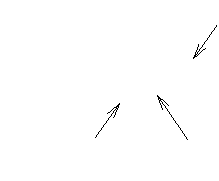
\includegraphics{getdp-sum}%
\end{picture}%
\setlength{\unitlength}{3947sp}%
%
\begingroup\makeatletter\ifx\SetFigFont\undefined%
\gdef\SetFigFont#1#2#3#4#5{%
  \reset@font\fontsize{#1}{#2pt}%
  \fontfamily{#3}\fontseries{#4}\fontshape{#5}%
  \selectfont}%
\fi\endgroup%
\begin{picture}(1742,1435)(2020,-4818)
\put(2020,-4668){\makebox(0,0)[lb]{\smash{\SetFigFont{10}{12.0}{\rmdefault}{\mddefault}{\updefault}{\color[rgb]{0,0,0}\small Geometrical}%
}}}
\put(2162,-4818){\makebox(0,0)[lb]{\smash{\SetFigFont{10}{12.0}{\rmdefault}{\mddefault}{\updefault}{\color[rgb]{0,0,0}\small entities}%
}}}
\put(3220,-4668){\makebox(0,0)[lb]{\smash{\SetFigFont{10}{12.0}{\rmdefault}{\mddefault}{\updefault}{\color[rgb]{0,0,0}\small Degrees of}%
}}}
\put(3321,-4817){\makebox(0,0)[lb]{\smash{\SetFigFont{10}{12.0}{\rmdefault}{\mddefault}{\updefault}{\color[rgb]{0,0,0}\small freedom}%
}}}
\put(3244,-3488){\makebox(0,0)[lb]{\smash{\SetFigFont{10}{12.0}{\rmdefault}{\mddefault}{\updefault}{\color[rgb]{0,0,0}\small Basis functions}%
}}}
\put(2176,-4036){\makebox(0,0)[lb]{\smash{\SetFigFont{10}{12.0}{\rmdefault}{\mddefault}{\updefault}{\color[rgb]{0,0,0}$f(\vec{x})=\sum_{i\in E}f_i w_i(\vec{x})$}%
}}}
\end{picture}
}

\end{slide}

\background{}{}{}

\begin{slide}

\begin{syntax}
\{ Name H1 ; Type Form0 ; \CC{discrete function space for H1}
  BasisFunction \{
    \{ Name wi ; NameOfCoef fi ; Function BF_Node ; \CC{order 1}
      Support Omega ; Entity NodesOf[ All ] ; \}
    \{ Name wi2 ; NameOfCoef fi2 ; Function BF_Node_2E ;  \CC{order 2}
      Support Omega ; Entity EdgesOf[ All ] ; \}
  \}
  Constraint \{
    \{ NameOfCoef fi ; \CC{cf. 'Constraint'}
      EntityType NodesOf ; NameOfConstraint Dirichlet ; \}
    \{ NameOfCoef fi2 ;
      EntityType NodesOf ; NameOfConstraint Dirichlet ; \}
  \}
\}
\end{syntax}

\end{slide}


% ---------------------------------------------------------------------------

\smallgetdp{fig/getdp-struct-jacobian.tex}

\chapter{\code{Jacobian}: defining jacobian methods}

\begin{slide}

\mybox{colbox}{11\semcm}{
  \begin{slideitemize}
  \item Mapping from reference to real space 
  \item Geometrical transformations (axisymmetric transformation, infinite
  domains, ...)
  \end{slideitemize}
}

\bigskip
\begin{syntax}
\{ Name Jacobian1 ;
  Case \{ \CC{piece-wise defined on groups}
    \{ Region OmegaInf; Jacobian VolSphShell \{Rint, Rext\}; \}
    \{ Region OmegaAxi; Jacobian VolAxi; \}
    \{ Region All; Jacobian Vol ; \}
  \}
\}
\end{syntax}

\end{slide}

% ---------------------------------------------------------------------------

\smallgetdp{fig/getdp-struct-integration.tex}

\chapter{\code{Integration}: defining integration methods}

\begin{slide}

\bigskip
\bigskip
\mybox{colbox}{11\semcm}{
  \begin{slideitemize}
  \item Various numeric and analytic integration methods
  \item Criterion-based selection
  \end{slideitemize}
}

\bigskip
\bigskip
\begin{syntax}
\{ Name Integration1 ; Criterion Test[]; \CC{combination of methods}
  Case \{ 
    \{ Type Gauss ;
      Case \{ \{ GeoElement Triangle ; NumberOfPoints 12; \}
             \{ GeoElement Tetrahedron; NumberOfPoints 15; \} \} \}
    \{ Type Analytic ; \}
  \} 
\}
\end{syntax}

\end{slide}

% ---------------------------------------------------------------------------

\smallgetdp{fig/getdp-struct-formulation.tex}

\chapter{\code{Formulation}: building equations}

\begin{slide}

\mybox{colbox}{11\semcm}{
  \begin{slideitemize}
  \item Various formulation types: FEM, BEM, circuit equations, ...
  \item Symbolic expression of equations: volume and surface integral
  terms, collocation
  \item Involves local, global and integral quantities based on function
  spaces
  \end{slideitemize}
}

\begin{syntax}
Equation \{
  Galerkin \{ DtDt [ epsilon[] * Dof\{e\} , \{e\} ]; ... \}
  Galerkin \{ [ 1/mu[] * Dof\{Curl e\} , \{Curl e\} ]; ... \}
\}
\end{syntax}

\rput(0.8\textwidth,6\semcm)
     {$\partial_t^2\ivol{\epsilon\vec{e}}{\vec{e}} + 
       \ivol{\mu^{-1}\Curl{\vec{e}}}{\Curl{\vec{e}}'}=0$}

\end{slide}

% ---------------------------------------------------------------------------

\smallgetdp{fig/getdp-struct-resolution.tex}

\chapter{\code{Resolution}: solving systems of equations}

\begin{slide}

\mybox{colbox}{10\semcm}{
  \begin{slideitemize}
  \item Description of a sequence of operations
  \item Time loops (with time step adaptation)
  \item Nonlinear iterative loops (e.g.\ fixed point or Newton-Raphson methods)
  \item Coupled problems (e.g.\ magneto-thermal coupling)
  \item Linking of various resolution steps (e.g.\ pre-computation of source
  fields) 
  \end{slideitemize}
}

\rput(0.8\textwidth,4\semcm){\parbox{12\semcm}{
\begin{syntax}
Operation\{\\
\hspace*{1em}InitSolution[A];\\
\hspace*{1em}TimeLoopTheta[tmin,tmax,dt,1]\{\\
\hspace*{2em}Generate[A]; Solve[A];\\
\hspace*{2em}If[Save[]]\{ SaveSolution[A]; \}\\
\hspace*{1em}\}\\
\}
\end{syntax}
}}

\end{slide}

% ---------------------------------------------------------------------------

\smallgetdp{fig/getdp-struct-postprocessing.tex}

\chapter{\code{PostProcessing}: exploiting computational data}

\begin{slide}

\mybox{colbox}{11\semcm}{
  \begin{slideitemize}
  \item ``Front-end'' to computational data
  \item Piece-wise definition of any quantity of interest
  \item Local or integral evaluation
  \end{slideitemize}
}

\bigskip
\begin{syntax}
Quantity \{
  \{ Name Induction;
    Value \{ Local \{ [ -mu[]*\{Grad phi\} ]; In Omega; \}
            Local \{ [ -\{dGreen\} ]; In BEM; \} \}
\}
\end{syntax}


\end{slide}

% ---------------------------------------------------------------------------

\smallgetdp{fig/getdp-struct-postoperation.tex}

\chapter{\code{PostOperation}: exporting results}

\begin{slide}

\mybox{colbox}{11\semcm}{
  \begin{slideitemize}
  \item Evaluation of post-processing quantities (e.g.\ maps, cuts, local or
  global evaluation, ...)
  \item Operations on post-processing quantities (sorting, smoothing,
  adaptation, ...) 
  \item Various output formats (e.g.\ space or time oriented, text, binary,
  ...) 
  \end{slideitemize}
}

\bigskip
\begin{syntax}
Print[ Induction, OnElementsOf Omega, File "b.pos", Format Gmsh ] ;
Print[ Induction, OnLine \{\{0,0,0\}\{1,0,0\}\} \{100\}, File "b.cut" ] ;
\end{syntax}

\end{slide}


\background{}{}{}

